\chapter{Organization: Development Process, Code Structure \& Contributing to MATSim}
\label{ch:developmentprocess}
% ##################################################################################################################

\hfill \textbf{Authors:} Andreas Horni, Kai Nagel, Marcel Rieser

\begin{center} 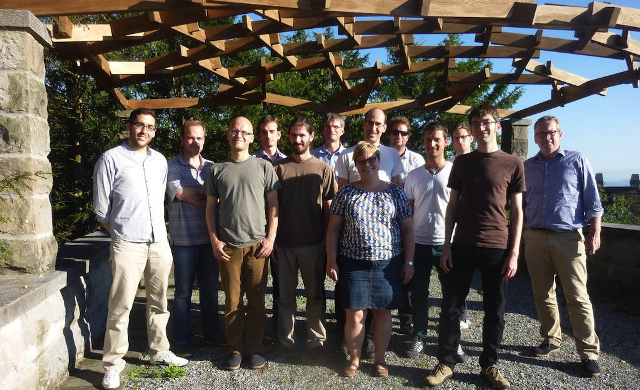
\includegraphics[width=0.5\textwidth, angle=0]{extending/figures/ConceptualMeetingVillaHatt.png} \end{center}

% ##################################################################################################################
This chapter describes how new functionality enters \gls{matsim}. It describes the \gls{matsim} team and community, the different roles existing in the \gls{matsim} project, development drivers and processes, and tools used for integration. The goal is to 
%give you 
provide an overview of the development process such that 
%you 
one quickly finds access to the \gls{matsim} community and such that 
%you are 
one is able to efficiently contribute to \gls{matsim} according to one role or another, if you commendably like to.

% ##################################################################################################################
\section{MATSim's Team, Core Developers Group, and Community}
The \imp{\gls{matsim} team}, 
%the heart of the \gls{matsim} community, 
currently consists of three research groups and a spin-off company, namely 
\begin{itemize}\styleItemize
\item the \gls{vsp} group at the \gls{ils}, \gls{tu} Berlin, led by Prof.~Dr.~Kai Nagel,
\item the \gls{vpl} group at the \gls{ivt}, \gls{eth} Zürich, led by Prof.~Dr.~Kay~W.~Axhausen, 
\item the recently founded Mobility and Transportation Planning group at the \gls{fcl}, based in Singapore and led by Prof.~Dr.~Kay~W.~Axhausen, and 
\item \gls{senozon}, based at Zürich with a subsidiary in Germany, founded by former \gls{phd} and research students. 
\end{itemize}

As common in research the universities groups' composition changes frequently. Over the last decade more than 50\,people build \gls{matsim} as listed earlier.

A small group of the \gls{matsim} team builds the \imp{\gls{matsim} core developers group} maintaining \gls{matsim}'s core as defined below in Section~\ref{sec:extending-core}.

Additionally, there is a \imp{\gls{matsim} community} composed of closely connected research groups (such as Stockholm, Pretoria, Poznan, and Jülich),
% and Toronto) 
%\kai{habe Toronto hier rausgenommen.  Spricht etwas dagegen?}
%\ah{nein. Danke! }
and more loosely connected external users coming together, \eg at the annual \gls{matsim} user meeting.   

\gls{matsim} is an open-source program provided by the \gls{gplv2}, thus, you are also very welcome to contribute to the code base as described in Section~\ref{sec:yourcontribution}. New contributors are mentored in the beginning \citep[][]{MATSIM-BecomingAContributor_Webpage_2015} to become familiar with the project and the coding conventions \citep[][]{MATSIM-CodingGuide_Webpage_2015}.

Picture~\ref{fig:team} shows a snapshot of the participants of the first conceptual meeting representing a good mix of team members but also associated researchers.
%
% ------------
\createfigure%
{Participants of the first MATSim conceptual meeting at Villa Hatt in Zürich in~2012}%
{Participants of the first MATSim conceptual meeting at Villa Hatt in Zürich in~2012}%
{\label{fig:team}}%
{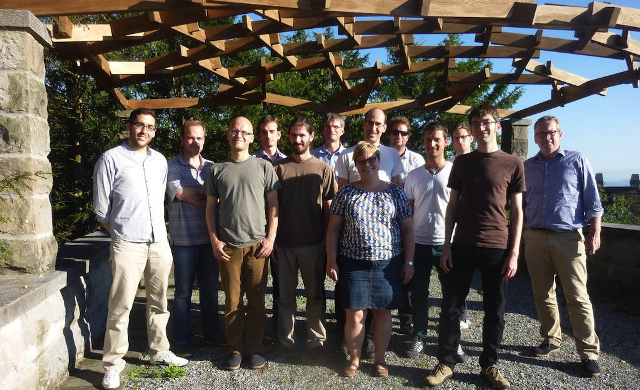
\includegraphics[width=0.99\textwidth, angle=0]{extending/figures/ConceptualMeetingVillaHatt.png}}%
{}
% ------------

% ##################################################################################################################
\section{Roles in the MATSim Community}
\label{sec:roles}
There are the following roles in the \gls{matsim} community.
%
\begin{itemize}\styleItemize
\item The \imp{\gls{matsim} user} uses the official releases or nightly builds and runs \gls{matsim} core with the \gls{configfile} (Section~\ref{sec:using-core-only}). He or she does not write computer code. Part~I of the book is dedicated to the \gls{matsim} user. On the web page he or she finds relevant information in the \emph{user's guide} and in the user's mailing list \lstinline|users@matsim.org|.
%
\item The \imp{\gls{matsim} power user} is a \gls{matsim} user with knowledge on how to use the additional modules presented in the book's part~II. He or she does \emph{not} program but knows how to use \gls{matsim} scripts as shown in Section~\ref{sec:writing-scripts-java}. Part~I and~II of the book are helpful to the \gls{matsim} power user.
%
\item The \imp{\gls{matsim} \gls{api} developer} extends \gls{matsim} by programming against the \gls{matsim} \gls{api} (Section~\ref{sec:writing-your-own-extensions}). He or she also finds his or her information in Part~II of the book, in particular in Chapter~\ref{ch:extensionpoints}, on the web page in the \emph{\gls{api} user's guide} and the \emph{developer's guide} and in the mailing list \lstinline|developers@matsim.org|.
%
%\item The \imp{\gls{matsim} \gls{api} developer} also programs against the \gls{matsim} \gls{api}, but additionally he or she is part of the \gls{matsim} code base by having his or her own playground or \gls{contribution} being part of the refactorings. 
%\ah{contribs auch, oder?} \kai{ja}. 
%The \gls{api} developer finds information in Part~II of this book, on the web page in the \emph{developer's guide} and in the mailing list \lstinline|developers@matsim.org| 
%
\item There are relatively few \textbf{\gls{matsim} core developers} stemming from the \gls{matsim} team, \ie the \gls{matsim} core developers group. This role is an extension of the \gls{matsim} \gls{api} developer and these guys make necessary modifications of the core as defined in Section~\ref{sec:extending-core}), usually after having discussed them in the issue tracker, in the \gls{matsim} committee, or at a developer meeting (see below). 
%% Part~II and part~III of this book might be particularly interesting for them.
%
% \kn{Sehe nicht, warum ausgerechnet die core developers neben dem software engineering auch noch die mathematisch-konzeptionelle Arbeit übernehmen müssen. --> weglassen}
% \ah{Dachte eher an Hintergrund: Damit man auch weiss, was man in einem weiteren Sinn eigentlich tut. Gibt aber verschiedene Blickwinkel drauf ... und deinen finde ich mittlerweile viel naheliegender.}
\end{itemize}
%
% ##################################################################################################################
\section{Code Base}
\label{sec:core-contribs-playgrounds}
The various pieces of \gls{matsim} are delineated by \gls{maven} projects and sub-projects. 
The \gls{maven} layout corresponds to the layout of the \gls{svn} repository.  
Note that the \gls{java} package structure does \emph{not} directly correspond to the \gls{maven}/\gls{svn} layout.

%---------------------------------------------------------------
\subsection{Main Distribution}
\label{sec:extending-main}
The ``\gls{matsim} main distribution'' corresponds to the ``matsim'' part of the \gls{svn} repository.% 
\footnote{
It is currently at \gls{sourceforge} under \url{https://svn.code.sf.net/p/matsim/source/matsim}. 
The exact path name sometimes changes, \eg because of changes at \gls{sourceforge}.
}

\gls{matsim} main distribution is maintained by the \gls{matsim} team.

At the time of writing, the \gls{matsim} main distribution contains following packages:
\begin{itemize}\styleItemize
\item \lstinline{org.matsim.analysis.*}
\item \lstinline{org.matsim.api.*} 
\item \lstinline{org.matsim.core.*}
%\footnote{Please note, that at the moment, the core is \emph{not} restricted to this large package as one might naturally assumes. \kai{chk.  Ich hatte das immer anders gesehen: core nur org.matsim.core.* und org.matsim.api.*.}}
\item \lstinline{org.matsim.counts.*} (see Section~\ref{sec:extending-counts})
\item \lstinline{org.matsim.facilities.*} (see Section~\ref{sec:extending-facilities})
\item \lstinline{org.matsim.households.*} (see Section~\ref{sec:extending-households})
\item \lstinline{org.matsim.jaxb.*}
\item \lstinline{org.matsim.lanes.*} presented in Chapter~\ref{ch:signalslanes}
\item \lstinline{org.matsim.matrices.*}
\item \lstinline{org.matsim.population.*}
\item \lstinline{org.matsim.pt.*} presented in Chapter~\ref{ch:pt}
\item \lstinline{org.matsim.run.*}
\item \lstinline{org.matsim.signalsystems.*} presented in Chapter~\ref{ch:signalslanes}
\item \lstinline{org.matsim.utils.*}
\item \lstinline{org.matsim.vehicles.*} (see Section~\ref{sec:extending-vehicles})
\item \lstinline{org.matsim.vis.*}
\item \lstinline{org.matsim.visum.*}
\item \lstinline{org.matsim.withinday.*} presented in Chapter~\ref{ch:withinday}
\item \lstinline{tutorial.*}
\end{itemize}

%---------------------------------------------------------------
\subsection{Core}
\label{sec:extending-core}
The material that is considered basic and indispensable residues in the three packages 
%Most of the core material is in packages that start with 
\begin{itemize}\styleItemize
\item \lstinline{org.matsim.api.*}
\item \lstinline{org.matsim.core.*}
\item \lstinline{org.matsim.run.*}
%% \item \lstinline{tutorial.*}
\end{itemize}
%
The \gls{matsim} core is maintained by the \gls{matsim} core developers group.

%\kai{Andreas, ich würde die tutorial package nicht zum core rechnen.  Es ist zwar richtig, dass das core team sich weitgehend darum kümmert.  Aber erstens hätte ich nichts dagegen, wenn das andere Leute übernehmen würden.  Und zweitens könnte man dann auch behaupten, dass jira zum Core gehört.}
%\ah{Ok. Hatte das, glaube ich, irgendwoher kopiert.}
 
%There is additional material in that part of the repository, for example under \lstinline{org.matsim.withinday.*} or \lstinline{org.matsim.pt.*}, that could as well be moved into the ``contrib'' section, but for the time being has remained in the core \ah{see below}, mostly because the maintainers of these parts have moved to \gls{senozon} and from there continue to maintain these functionalities.

%\ah{we should make the difference more clearer between \lstinline{org.matsim.core.*} and \lstinline{org.matsim.*}. 
% I have the impression that we use the word ``core'' interchangeably, and even if not, then having \lstinline{org.matsim.core.*} inside ``core (?) MATSim'' is confusing.}
%\ah{see now below and issues \url{https://matsim.atlassian.net/browse/MATSIM-327} and \url{https://matsim.atlassian.net/browse/MATSIM-323}}

%---------------------------------------------------------------
\subsection{Contribs}
The idea of the \glspl{contribution} part of the repository is to host community contributions considered helpful. 
Historically, most contributors are from \gls{matsim} team, but this is not a requirement.
The code is maintained by the corresponding contributor. 
Code is considered much more stable than the one within playgrounds as shown below.%
\footnote{
It is currently at \gls{sourceforge} under \url{https://svn.code.sf.net/p/matsim/source/contrib}.  
}
The \gls{java} packages often have the root \lstinline{org.matsim.contrib.*}, but this is not enforced.

At the time of writing, following \glspl{contribution} are in the ``contrib'' repository:
\begin{itemize}\styleItemize
\item \lstinline{org.matsim.contribs.accessibility.*} presented in Chapter~\ref{ch:accessibility}
\item \lstinline{org.matsim.contribs.analysis.*} presented in Section~\ref{sec:contrib-analysis}
\item \lstinline{org.matsim.contribs.cadytsIntegration.*} presented in Chapter~\ref{ch:cadyts}
\item \lstinline{org.matsim.contribs.dvrp.*} presented in Chapter~\ref{ch:dts}
\item \lstinline{org.matsim.contribs.emissions.*} presented in Chapter~\ref{ch:emissions}
\item \lstinline{org.matsim.contribs.freight.*} presented in Chapter~\ref{ch:freight}
%\item \lstinline{org.matsim.contribs.freightChains.*} \ah{gehört zu freightChainsFromTravelDiaries}
\item \lstinline{org.matsim.contribs.freightChainsFromTravelDiaries.*} presented in Section~\ref{sec:freightChainsFromTravelDiaries}
\item \lstinline{org.matsim.contribs.grips.*} presented in Chapter~\ref{ch:evacuation}
\item \lstinline{org.matsim.contribs.gtfs2matsimtransitschedule.*} presented in Section~\ref{sec:SemiTool}
\item \lstinline{org.matsim.contribs.locationchoice.*} presented in Chapter~\ref{ch:destinationchoice}
\item \lstinline{org.matsim.contribs.matrixbasedptrouter.*} presented in Section~\ref{sec:matrix-based-pt-router}
\item \lstinline{org.matsim.contribs.matsim4urbansim.*} presented in Section~\ref{sec:matsim4urbansim}
\item \lstinline{org.matsim.contribs.minibus.*} presented in Chapter~\ref{ch:pt}
\item \lstinline{org.matsim.contribs.multimodal.*} presented in Chapter~\ref{ch:multimodalsim}
\item \lstinline{org.matsim.contribs.networkEditor.*}\footnote{This contribution is not presented in the book. Instead, two external editors also developed by MATSim team members are presented in Chapter~\ref{ch:networkeditor}} %presented in Chapter~\ref{ch:networkeditor} \ah{afaik: the 2 presented ones are external}
\item \lstinline{org.matsim.contribs.otfvis.*} presented in Chapter~\ref{ch:otfvis}
\item \lstinline{org.matsim.contribs.parking.*} presented in Chapter~\ref{ch:parking}
\item \lstinline{org.matsim.contribs.roadpricing.*} presented in Chapter~\ref{ch:roadpricing}
%\item \lstinline{org.matsim.contribs.signals.*} presented in Chapter~\ref{ch:signalslanes} \ah{only a placeholder}
\item \lstinline{org.matsim.contribs.transEnergySim.*} presented in Chapter~\ref{ch:elvehicles}
\item \lstinline{org.matsim.contribs.wagonSim.*} presented in Chapter~\ref{ch:wagonSim}
\end{itemize}

%% in the code base 
%% as \gls{matsim} contributions (\lstinline|package org.matsim.contrib.*|). Such modules are usually provided by \gls{matsim} \gls{api}-users or developers. %

%---------------------------------------------------------------
\subsection{Playgrounds}
Another element of the \gls{matsim} repository are the ``playgrounds''. 
These are meant as a service to programmers. 
The have historically grown from the fact that \gls{matsim}'s object classes and in consequence the interfaces between them have evolved and grown over time, and thus a stable \gls{api} was not available.  
At this point, the extension points described in Chapter~\ref{ch:extensionpoints} should be somewhat stable, and development against them should be possible without major changes from release to release.  
Anybody who needs tighter integration with the project should apply for a playground of her or his own.

% ====================================================================================
\subsection{Contributions and Extensions}
Congruent with the structure of this book, the \gls{matsim} code structure contains a core which allows to run basic \gls{matsim} using the \gls{configfile}, a population and a network. Packages going beyond this basic functionality are \glspl{extension}, where three different kind of extensions exist:
\begin{itemize}\styleItemize 
\item Extensions in main distribution.%
\footnote{At time of writing it is unclear if these extensions should be made \glspl{contribution} one day, shrinking \gls{matsim} main distribution to its core.
}
\item Extensions contributed by \gls{matsim} community known as \glspl{contribution}.
\item Any code written anywhere published or unpublished extending \gls{matsim} core.
\end{itemize}
Extensions are listed at \url{http://matsim.org/extensions}.

% ====================================================================================
\subsection{Releases, Nightly Builds and Code HEAD}
\label{sec:releases-builds}
Twice a year, a \gls{matsim} release is published, which can be downloaded from \gls{sourceforge} at \url{http://sourceforge.net/projects/matsim/files/}. Usually, \gls{matsim} users and \gls{matsim} power users as defined above in Section~\ref{sec:roles} work with releases. 

MATSim is based on continuous integration and, thus, nightly builds are available without stability guarantee \url{http://matsim.org/downloads/nightly}. Nightly builds might be used by \gls{matsim} \gls{api} developers, which depend on a very recent feature. 

\gls{matsim} \gls{api} developers or core developers often work on the code's HEAD version, which is available from \gls{sourceforge} at \url{http://sourceforge.net/p/matsim/source/HEAD/tree/}.

Nightly builds are only generated when the code compiles and passes the regression tests.  They are, in consequence, somewhat ``safer'' than the direct download from the HEAD.

% ##################################################################################################################
\section{Drivers, Organization and Tools of Development}
Main drivers of the \gls{matsim} development are the projects and dissertations of the \gls{matsim} team. 
New features are developed as an answer to requirements of these dissertations and projects, where projects range 
%
from purely scientific ones (often sponsored by \gls{snf} or \gls{dfg}) 
%
via projects for governmental entities
%administration 
%
and projects where science and industry contribute equally (\eg \gls{cti}-projects) 
%
to purely 
%industrial 
commercial projects, which are managed by \gls{senozon} in the majority of cases. 
%
A significant amount of innovation is also introduced by the collaboration with external researchers.

Systematic code integration is mainly performed by the Berlin group and by \gls{senozon}. 
This includes continuous code review and integration upon request of the community, but also comprehensive code refactorings to clean up
%degenerated 
code and to 
improve modularity.  Refactorings are discussed and documented in the \gls{matsim} issue tracker.

The development process is supported by a standing \gls{matsim} committee discussing conceptual issues on a regular basis. 
Another element bringing in innovation but also organization are the annual meetings. 
Right from the beginnings, there has been a \gls{matsim} developer meeting focused on coding issues. 
Later, a user meeting giving insights into current work by the community has been invented. 
Finally, a conceptual meeting has been added strictly dedicated to issues that go beyond pure software engineering. 
The developer and the conceptual meeting have shown to establish an effective road map, which has guided the development for the remainder of the year. 

The internal development is organized by regular group meetings, in Zürich for example by the \gls{matsim} ``group meeting''.
%% and in Berlin by the "jour fix". 

Due to the heterogeneous character of the community and its individual research groups, with every member being engaged in his individual dissertation work, organizing the development in an agile and somewhat ad hoc manner has been regarded beneficial over adopting an established and strict software project management method.

% ====================================================================================
%\subsection{Development Tools}
%\kai{Moved some material from here to ``history''.}
%\ah{ok. Adapted title, as there was nothing about "core" here anyamore.}

\gls{matsim} development makes use of a whole bunch of tools greatly leading to better software quality. Summarized and accessible from \url{http://matsim.org/developer}:
%---with private access---
%
%m.E. war das nie non-public.  Evtl. nicht auf der home page ausgewiesen. kai, dec'14
a change log, an issue tracker, the \gls{javadoc}, static code analyses performed by \emph{FindBugs} and \emph{PMD}, test code coverage analysis, copy paste analysis, code metrics, \gls{maven} dependencies, the complete code linked by \gls{xref}, and the information about the nightly test results are provided. These nightly test results are generated by the \gls{matsim} build server based on \gls{jenkins}. 

Furthermore, there is a \gls{matsim} benchmark available in the user's guide and at \url{http://matsim.org/files/benchmark/benchmark.zip}.
}
%\url{http://www.matsim.org/docs/devguide/optimization}. \kai{link funktioniert nicht.  Wir hatten neulich schon danach gefahndet, aber das Material ist einfach in den latex user guide gewandert.  Der Benchmark selber ist unter \url{http://matsim.org/files/benchmark/benchmark.zip}.}
%\ah{danke}

Most \gls{matsim} developers use \gls{eclipse} as an \gls{ide}. The \gls{matsim} documentation is tailored to this \gls{ide}. Team development is based on \gls{svn}. External libraries dependencies are managed by \gls{maven}.

% ##################################################################################################################
\section{Documentation, Dissemination and Support}
The main documentation can be found on the \gls{matsim} web page \citep[][]{MATSIM-Docu_Webpage_2015}, where information is provided in the three guides mentioned above. Additionally, a handful of tutorials is available, with the ``Quickstart''-tutorial to give fast access to \gls{matsim} and the ``Learning \gls{matsim} in 8\,Lessons''-tutorial, which is used for the user's meetings and hands-on tutorials in Berlin, Zürich and occasionally elsewhere, also listed on that page. 

Code documentation in form of \gls{javadoc} can be found unter \url{http://matsim.org/javadoc}, 
%at \citet[][]{MATSIM-Javadoc_Webpage_2015}, 
as \gls{xref} view \url{http://matsim.org/xref} and as doxygen documentation \url{http://matsim.org/doxygen}. %\kai{gerne auch xref und doxygen URLs: \url{http://matsim.org/xref} and \url{http://matsim.org/doxygen}.}

For fast application of \gls{matsim} some small-scale example scenarios are provided in the code base (\lstinline|folder: examples|), where recently an extended version of the well-known benchmark scenario for the City of Sioux Falls has been added \citep[][]{ChakirovFourie_TechRep_FCL_2014} (Chapter~\ref{ch:siouxfalls}). %\kai{Auf den test input folder sollte m.E.\ auf keinen Fall verwiesen werden ... test inputs bleiben normalerweise auf dem Status, mit dem sie erstellt wurden, passen sich also nicht an neue Entwicklungen an.  Stattdessen bitte ``folder: examples''.} \ah{danke}

Further information is disseminated at the afore-described annual user meetings and \gls{matsim} mailing lists \url{http://www.matsim.org/mailinglists}. Usually, also support is provided by the \gls{matsim} team via these mailing lists. Particularly active in support are the Berlin group and \gls{senozon}. A theoretical overview of all the components in \gls{matsim} is given by the numerous papers published in international journals and presented at worldwide conferences; an overview can be found at \citep[][]{MATSIM-Publications_Webpage_2015} and in this book's part~II.

The information on \gls{matsim} is quite extensive, however, getting a complete picture as a new \gls{matsim} user or developer requires a substantial literature search. Minimization of this effort is the goal of the book at hand.

% ##################################################################################################################
\section{Your Contribution to MATSim}
\label{sec:yourcontribution}
The technical details, \ie the \gls{matsim} extensions points, where to hook with \gls{matsim} are detailed in the next chapter. Here, the different ways of contributing to \gls{matsim} according to the roles presented in Section~\ref{sec:roles} are introduced.

As a \gls{matsim} user, power user, or \gls{api} developer, you are warmly welcome to make an important impact by reporting your achievements, needs and problems with, or bugs of, the software via the users mailing list or at the annual \gls{matsim} user meeting. 

If you would like to directly contribute to the code base of \gls{matsim} you are welcome to become part of the \gls{contribution} repository.

If you are the type of guy that likes to change the core system, you can, although it is a long way, become a member of the \gls{matsim} core developers group. Core developers are usually picked from the \gls{matsim} team. Prerequisites are a strong computer scientist background, several years of experience with \gls{matsim} and a deep understanding of large software projects.

% ##################################################################################################################
%\section{Discussion and TODOs}
%\label{sec:development_process}
%Will be commented, when chapter is finished. Make final results traceable.
%
%% --------------
%\kai{Ich würde gerne ``Development process'' und ``Contributing to MATSim'' auftrennen.  Ersteres beschreibt Dinge wie core development, regression tests, etc.  Aber ``contributing to MATSim'' sollte sich auf die extension points konzentrieren.  Vielleicht zusammen mit dem vorhergehenden Kapitel.}
%
%\kai{Bin mir allerdings beim zweiten Nachdenken nicht mehr sicher, ob das so kategorisch sein muss.  Wir sollten erstmal versuchen, ``contributing to matsim'' als logische Folge des development process zu schreiben.  Dann sind ``minimally invasive contributions'' ja gerade solche, welche die extension points verwenden.}
%
%% --------------
%\ah{Vieles noch etwas zu implizit dargestellt! -> Aufzählungen einfügen. Playgrounds! Testing! Verantwortlichkeiten!}
%
%% --------------
%\ah{Classes und Methods stabil seit Langem: 
%auf was deutet das hin? Zu wenig Innovation oder Clean-Code? Steckt zuviel in den Playgrounds, Contribs oder ist das genau richtig?
%Wurde Kernfunktionalität eingefügt und dafür weniger Zentrales (wie Evacuation) nach und nach in Contrib verschoben?}
%
%\ah{Der Drop Ende 2007, war das schon Core, API Umstruktutierung oder war das die Entfernung von G. package?}
%\kai{Entfernung von Gunnar's package.}
%
%\createfigure%
%{Code development since 2005}%
%{Code development since 2005}%
%{\label{fig:codedev}}%
%{%
  %\createsubfigure%
  %{...}%
  %{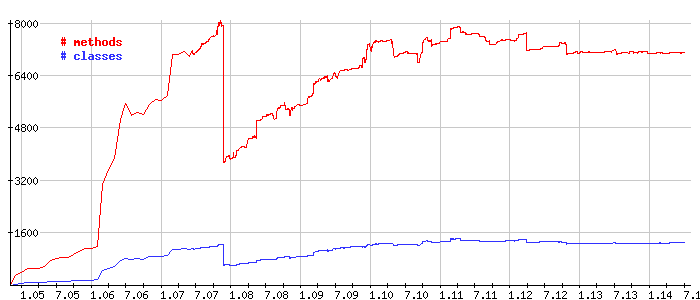
\includegraphics[width=0.95\textwidth,angle=0]{extending/figures/nof_classes.png}}%
  %{\label{fig:codedev0}}%
  %{}%
  %\createsubfigure%
  %{...}%
	%{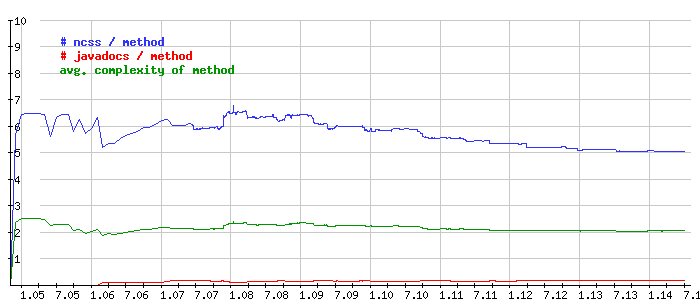
\includegraphics[width=0.95\textwidth,angle=0]{extending/figures/avg_method.png}}%
  %{\label{fig:codedev1}}%
  %{}%
%}%
%{}
%
%
%\ah{noch weiter eingehen auf Code Struktur? Resources, XML, ect.???}
%\ah{approx. number of playgrounds}
%\ah{approx number of code lines /classes at the different locations (core, playgrounds, contributions etc.}

% ##################################################################################################################
% Local Variables:
% mode: latex
% mode: reftex
% mode: visual-line
% TeX-master: "../main"
% comment-padding: 1
% fill-column: 9999
% End: 
